%!TEX root = rapport.tex
\newpage

\section{Evaluation of existing visualizations in lambda theory}
According to our research, nothing exactly similar to our theses exist. There does on the other hand exist visualizations of other lambda-related areas. In this section we will discuss these.

\subsection{Alligator Eggs -  A Puzzle Game by Bret Victor}
\begin{align*}
	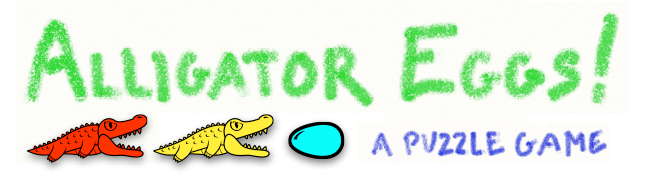
\includegraphics[scale=0.5]{AlligatorEggs.png}	
\end{align*}
The ``Alligator Eggs -  A Puzzle Game'' is a fun and children-like way of visualizing the computation of a lambda term. It self and is not directly related to our thesis concerning evaluation of the $\beta$-reduction-graphs of the lambda term.\\

The theory in this game is based on the untyped lambda calculus. The game rules is defined according to the following:
\begin{enumerate}
	\item A hungry alligator is a lambda abstraction
	\item An old alligator is parentheses
	\item Eggs are variables
	\item The eating rule corresponds to a $\beta$-reduction
	\item The color rule corresponds to alpha-conversion
	\item The old age rule says that if a pair of parentheses contains a single term, the parentheses can be removed\\\\
\end{enumerate}

In the example below we the eating rule in use. The green alligator will whatever is in front of it. In this case it will eat the yellow alligator and its yellow egg. After the green alligator has eaten the yellow alligator and egg it will die and its egg will hatch into what it has eaten. The miracle of life, as the author calls it. This little episode is, as stated in the definition, corresponding to a $\beta$-reduction. 

\begin{align*}
	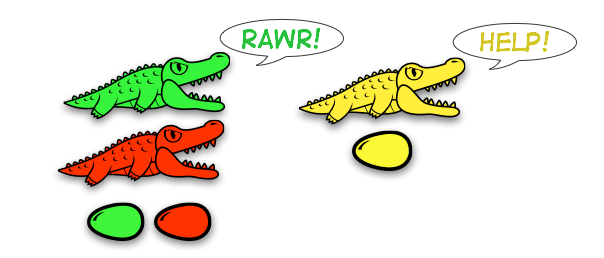
\includegraphics[scale=0.5]{alligatorEat.png}	
\end{align*}

The ``Alligator Eggs -  A Puzzle Game'' does not deal with the same lambda theory as we do in our theses. It does although deal with being visually attractive. The figures and colors in the game makes lambda calculus attractive even for very young kids.

The ``Alligator Eggs -  A Puzzle Game'' has also been implemented 


\subsection{Lambda Animator by Mike Thyer}
The ``Lambda Animator'' by Mike Thyer is a bla bla bla....




% subsubsection subsubsection_name (end)
% The untyped lambda calculus was introduced in 1936 by Alonzo Church
% [reference] as part of the search for a solid foundation for mathematics. It is
% heavily intertwined with the notion of a ``function'', in the sense that logic
% and mathematics is represented with only functions and untyped variables that
% can be either free or bound.


% alt er funktioner
% eksempler
